\documentclass[xcolor=table, handout]{beamer}

\usepackage{shyne}

% Theme settings
\setbeamertemplate{navigation symbols}{}

\usetheme{Madrid}
\usefonttheme{structurebold}
\usefonttheme[onlymath]{serif}

\AtBeginSection[]
{ 	\begin{frame}{}

	{
	\usebeamerfont{frametitle}
	\begin{beamercolorbox}
		[wd={\textwidth}, center, sep=.2in, rounded=true, shadow=true]
		{frametitle}
	Chapter \thesection\\  \secname 
	\end{beamercolorbox}
	}
	
	\end{frame} 
}

\AtBeginSubsection[]
{ 	\begin{frame}{}

	{
	\usebeamerfont{frametitle}
	\begin{beamercolorbox}
		[wd={\textwidth}, center, sep=.2in, rounded=true, shadow=true]
		{frametitle}
	Section \thesection .\thesubsection\\  \subsecname 
	\end{beamercolorbox}
	}
	
	\end{frame} 
}

\title[Chapter 8]{Stat 201: Statistics I\\ Chapter 8 }
\author[M. Shyne]{}
\institute[Metro State]{
\includegraphics[width=1.75in]{../images/metro_logo}}
\date[Mar 19, 2018]{March 19, 2017
\\ \bigskip \bigskip 
\includegraphics[width=.4in]{../images/cc_big}}


\begin{document}
\frame{\titlepage}

% Chapter 8
\setcounter{section}{7}
\section{Hypothesis Testing}

% Section 8.1
\subsection{Basics of Hypothesis Testing}

\begin{frame}{Statistical inference}
\begin{block}{}
\large
Previously, statistics from random samples were used to learn something about populations by estimating population parameters. ``Truths" about populations were inferred from the data of the sample.\\
\medskip
A similar question can be posed: Is a sample drawn from a population that is the same in an important way to a known population, or is the sample drawn from a population that is significantly different?
\end{block}

\end{frame}


\begin{frame}{Hypothesis tests}
\begin{block}{}
\large An \bt{hypothesis test} is a formal statistical procedure to test claims about population parameters based on samples drawn from populations. Such claims, or \bt{hypotheses}, are often written as simple mathematical statements.\\
\medskip
It is important to be clear as to which population the claims or the tests are about,
\end{block}
\end{frame}

\begin{frame}{Hypotheses, example}
\begin{exampleblock}{Example}
\large
\begin{itemize}
\item Male Metro State students are shorter on average than the national mean of 69.2 inches.
\begin{itemize}
\pause\item Population: Male Metro State students
\pause\item $\mu < 69.2$
\end{itemize}

\pause\item The proportion of teen drivers who text or email while driving is 40\%
\begin{itemize}
\pause\item Population: Teen drivers
\pause\item $p = 0.4$
\end{itemize}

\pause\item A patient diagnosed with a particular rare disease has an expected survival time of 36 months. A new experimental treatment will extend the survival time.
\begin{itemize}
\pause\item Population: Patients with disease on experimental treatment
\pause\item $\mu > 36$
\end{itemize}
\end{itemize}
\end{exampleblock}
\end{frame}

\begin{frame}{Hypotheses}
\begin{block}{}
\large
The first step to conduct an hypothesis test is to identify two hypotheses.
\end{block}
\pause
\begin{block}{}
{\large The \bt{null hypothesis} is the claim that nothing interesting has occurred, that a sub-population is \bt{not} different than the general population or that population parameters did \bt{not} change after treatment. }
\end{block}
\pause
\begin{block}{} 
\large Conversely, the \bt{alternative hypothesis} is the claim that something interesting has occurred, that a sub-population is different or that parameters did change after treatment.
\end{block}
\end{frame}

\begin{frame}{Hypotheses, cont.}
\begin{block}{}
Null hypothesis:
\begin{itemize}
\item Denoted by $\bv{H_0}$
\item Always a statement that a parameter is \bt{equal to} some value
\item That value, denoted $p_0$ or $\mu_0$, is called the proportion or mean under the null hypothesis
\end{itemize}
\end{block}
\pause
\begin{block}{}
Alternative hypothesis:
\begin{itemize}
\item Denoted by $\bv{H_1}$ or $\bv{H_a}$ 
\item Can be a statement that a parameter is \bt{less than}, \bt{greater than} or \bt{not equal to} some value
\item Is usually a statement representing the research question
\end{itemize}
\end{block}
\end{frame}

\begin{frame}{One-sided vs. two sided tests}
\begin{block}{}
\large If an alternative hypothesis has the form of a parameter being less than or greater than some value, the hypothesis test is called a \bt{one-sided test}.\\
\medskip
If an alternative hypothesis has the form of a parameter being not equal to some value, the hypothesis test is called a \bt{two-sided test}.
\end{block}
\end{frame}

\begin{frame}{Hypotheses, example}
\begin{exampleblock}{Example}
\large
Identify the null and alternative hypotheses, and whether it is a one-sided or two-sided test.\\
\pause\medskip
In the United States, adult men have a mean height of 69.2 inches. The Metro State administration want to do a study to see if male Metro State students are shorter than the general US population.

\begin{itemize}
\pause\item $H_0: \mu = 69.2 \qquad H_a: \mu < 69.2$\qquad One-sided

\end{itemize}

\pause\medskip
A patient diagnosed with a particular rare disease has an expected survival time of 36 months. A clinical trial is conducted to see if a new experimental treatment will change the survival time.
\begin{itemize}
\pause\item $H_0: \mu = 36 \qquad H_a: \mu \ne 36$\qquad Two-sided
\end{itemize}

\end{exampleblock}
\end{frame}

\begin{frame}{Structure of hypothesis tests}
\begin{block}{}
\large
Starting with null and alternative hypotheses derived from the research question and a random sample, all hypothesis tests have the same basic structure.
\begin{itemize}
\pause\item A test statistic is calculated which indicates the location of the sample within the sampling distribution, assuming the null hypothesis is true.

\pause\item The probability of getting a test statistic equal to or more extreme than the statistics belonging to the sample is calculated.

\pause\item If the calculated probability is below a pre-specified threshold, the null hypothesis is \bt{rejected} and it is said that there is evidence to support the alternative hypothesis.

\pause\item If the calculated probability is not below the pre-specified threshold, the null hypothesis is \bt{not rejected} and it is said that there is not evidence to support the alternative hypothesis.
\end{itemize}
\end{block}
\end{frame}

\begin{frame}{P-values}
\begin{block}{}
\large In a hypothesis test, the \bt{p-value} is the probability of getting a sample with the test statistic or one more extreme, assuming the null hypothesis is true.
\begin{itemize}
\item Not to be confused with the population proportion $p$ or the probability function $P(A)$, though a p-value does represent a probability.
\end{itemize} 
\end{block}
\medskip
{\centering
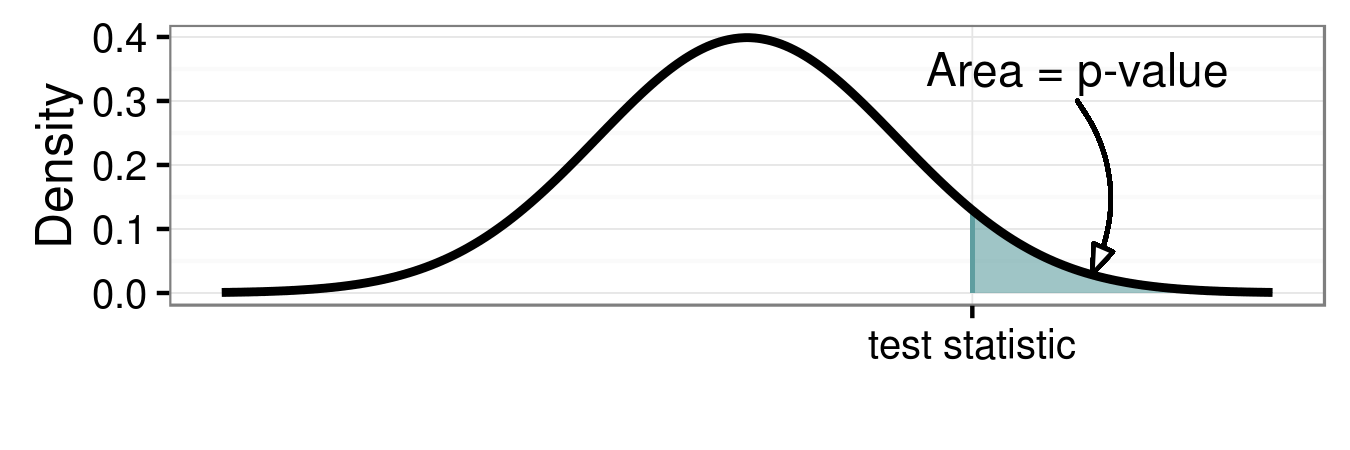
\includegraphics[width=4.5in]{../images/ch08_pvalue}
\par}

\end{frame}

\begin{frame}{Calculating p-values}
\begin{block}{}
\large
Calculating a p-value is that same as calculating probabilities in sampling distributions already learned.
\begin{itemize}
\pause\item Identify sampling distribution: 
\begin{itemize}
\item $z$ distribution for proportions
\item $t$ distribution for means
\end{itemize}
\pause\item Calculate \bt{test statistic}: $z$-score or $t$-score
\pause\item Find probability of test statistic or more extreme values in sampling distribution
\pause\item That probability is the p-value
\end{itemize}
\end{block}

\begin{block}{}
\large
Luckily, all these steps can be accomplished easily with technology.
\end{block}
\end{frame}

\begin{frame}{Significance level}
\begin{block}{}
\large Once the p-value is calculated, it is compared against a pre-specified threshold. This threshold is called the \bt{significance level} of the test.
\begin{itemize}
\pause\item Denoted by $\bv \alpha$
\pause\item This is the same $\alpha$ used for critical values and confidence intervals
\pause\item Thus, significance level can be thought of as an area in a sampling distribution
\pause\item Sometimes referred to as the rejection region
\end{itemize}
\end{block}
\end{frame}

\begin{frame}{Significance level for one-sided test}
\begin{block}{}
\large
In a one-sided test, the entire rejection region is located at one end of the distribution or the other.
\end{block}
{\centering
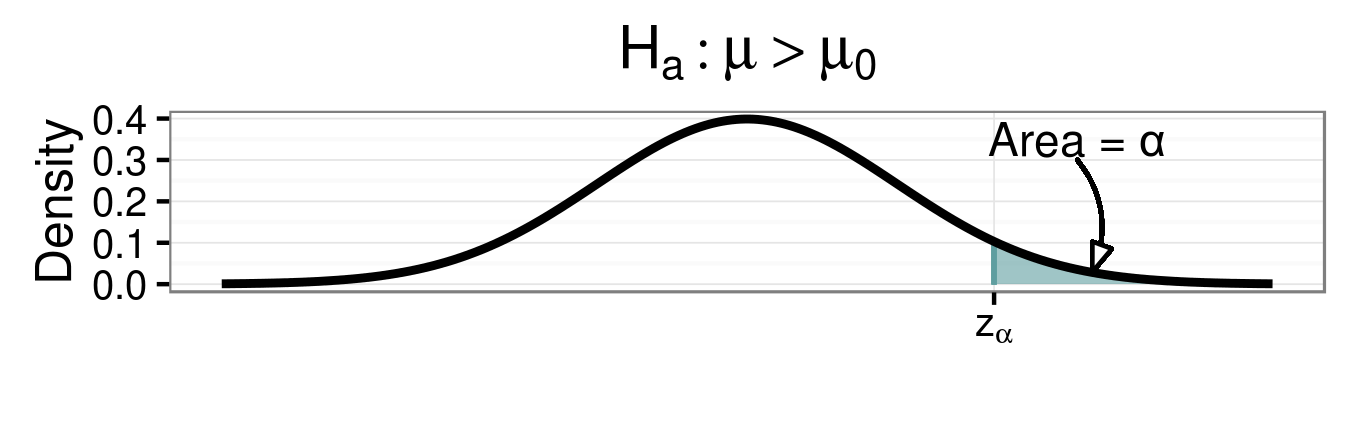
\includegraphics[width=4.5in]{../images/ch08_sig_up}
\par}
{\centering
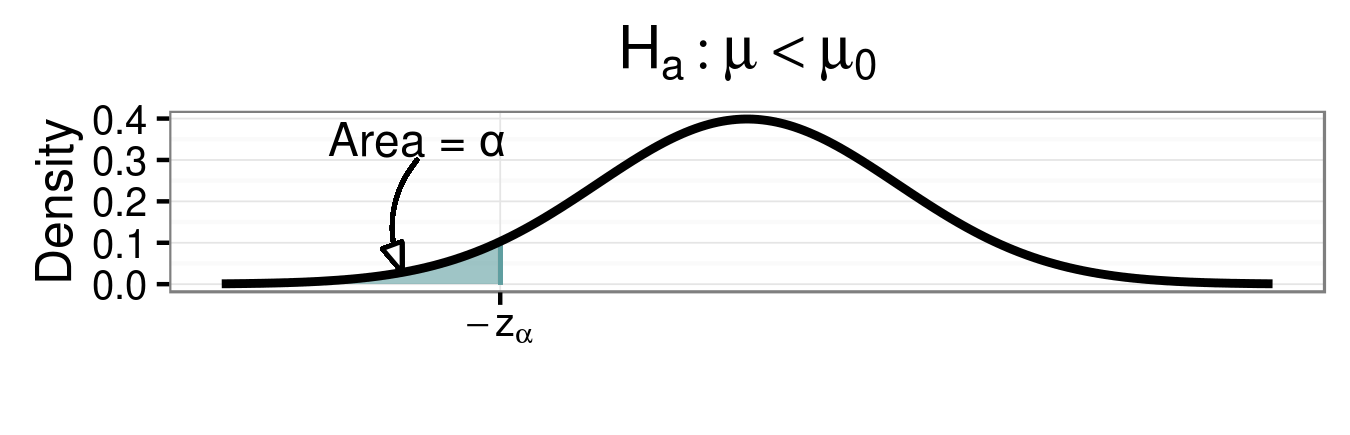
\includegraphics[width=4.5in]{../images/ch08_sig_low}
\par}

\end{frame}

\begin{frame}{Significance level for two-sided test}
\begin{block}{}
\large
In a two-sided test, the rejection region is split between the lower and upper extremes of the distribution.
\end{block}
\bigskip
{\centering
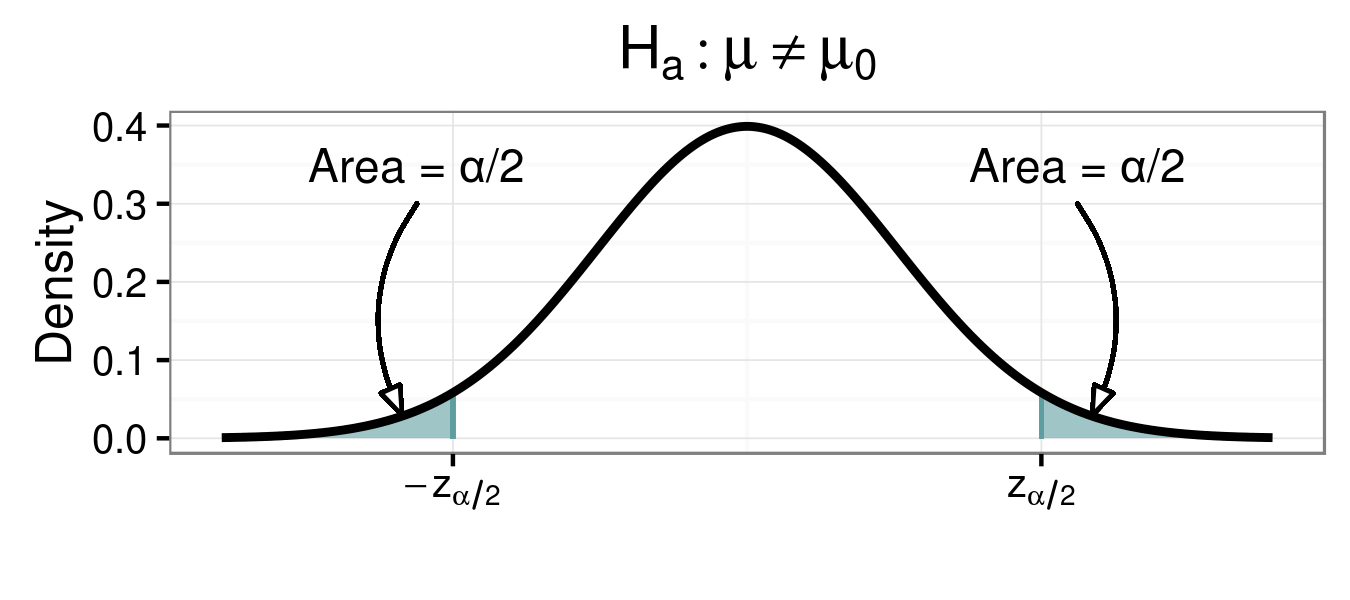
\includegraphics[width=4.5in]{../images/ch08_sig_2}
\par}

\end{frame}


\begin{frame}{Stating conclusions}
\begin{block}{}
\large
When reporting the results of an hypothesis tests, the following elements should be included:
\begin{itemize}
\pause\item Report the test statistic and p-value
\pause\item Report a decision on the null hypothesis based on the p-value and significance level ($\alpha$). 
\begin{itemize}
\item State the decision as ``Reject $H_0$" or ``Do not reject $H_0$".
\item The null hypothesis is never ``accepted".
\end{itemize}
\pause\item State the conclusion in terms of the research question
\begin{itemize}
\item ``There is evidence for..."
\item ``There is not evidence for..."
\end{itemize}
\end{itemize}
\end{block}
\end{frame}

\begin{frame}{Stating conclusions, example}
\begin{exampleblock}{Example}
\large
A study is conducted to test the claim that male Metro State students are shorter than the general population height of 69.2 inches. The test at a $\alpha=0.05$ level of significance produces a test statistic $t=-1.859$ and a p-value of $0.0358$. State the conclusion of the test.
\begin{itemize}
\pause\item $H_0: \mu=69.2, \qquad H_a: \mu < 69.2$
\pause\item $p=0.0358 < \alpha = 0.05$. Reject the null hypothesis. There is evidence to conclude that male Metro students are shorter than the general population.
\end{itemize}
\end{exampleblock}
\end{frame}

\begin{frame}{Stating conclusions, example}
\begin{exampleblock}{Example}
\large
A patient diagnosed with a particular rare disease has an expected survival time of 36 months. A clinical trial is conducted to see if a new experimental treatment will change the survival time. The hypothesis test at $\alpha = 0.01$ level of significance produces a p-value of 0.098. State the conclusion of the test.
\begin{itemize}
\pause\item $H_0: \mu = 36 \qquad H_a: \mu \ne 36$
\pause\item $p=0.098 > \alpha = 0.01$. Do not reject the null hypothesis. There is not evidence to conclude that the experimental treatment changes survival time.
\end{itemize}\end{exampleblock}
\end{frame}

\begin{frame}{Steps for hypothesis test}
\begin{block}{}
\large
\begin{enumerate}
\item Identify null and alternative hypotheses from research question
\item Determine appropriate sampling distribution
\item Calculate test statistic
\item Calculate p-value
\item Compare p-value to significance level $\alpha$ and report decision
\item State conclusion in terms of original research question
\end{enumerate}
Note: Steps 3 and 4 are often accomplished with technology
\end{block}
\end{frame}

\begin{frame}{Making a decision with p-value}
\begin{block}{}
\large
A \bt{small} p-value ($p < \alpha$) means a low probability of getting the observed sample if the null hypothesis is true. Thus, the null hypothesis is rejected.\\
\medskip
A \bt{large} p-value ($p > \alpha$) then means that the sample is not unlikely under the null hypothesis. Thus, the null hypothesis is not rejected.
\end{block}

\pause
\begin{alertblock}{To remember\ldots}
\Large If p is low, the null must go.
\end{alertblock}

\end{frame}

\begin{frame}{Or if this helps\ldots}

{\centering

\includegraphics[width=2.5in]{../images/ch08_p_value_meme}
\par}

\end{frame}

\begin{frame}{Critical value method}
\begin{block}{}
\large
The hypothesis test procedure discussed thus far is known as the p-value method. An alternative method, known as the \bt{critical value} method, does not use p-values, but rather compares test statistics directly to appropriate critical values. If the test statistic is more extreme than the critical value, the null hypothesis is rejected.
\end{block}
\end{frame}

\begin{frame}{Critical value method, example}
\begin{exampleblock}{Example}
\large
A two-sided test with $\alpha = 0.05$ level of significance is conducted and results in a test statistic $z= - 2.8$.
\begin{itemize}
\item Recall, critical value $z_{\alpha/2} = \pm 1.96$.
\item Since $-2.8$ is more extreme than $-1.96$ ($-2.8 < -1.96$), reject the null hypothesis.
\end{itemize} 
\end{exampleblock}

\medskip
{\centering
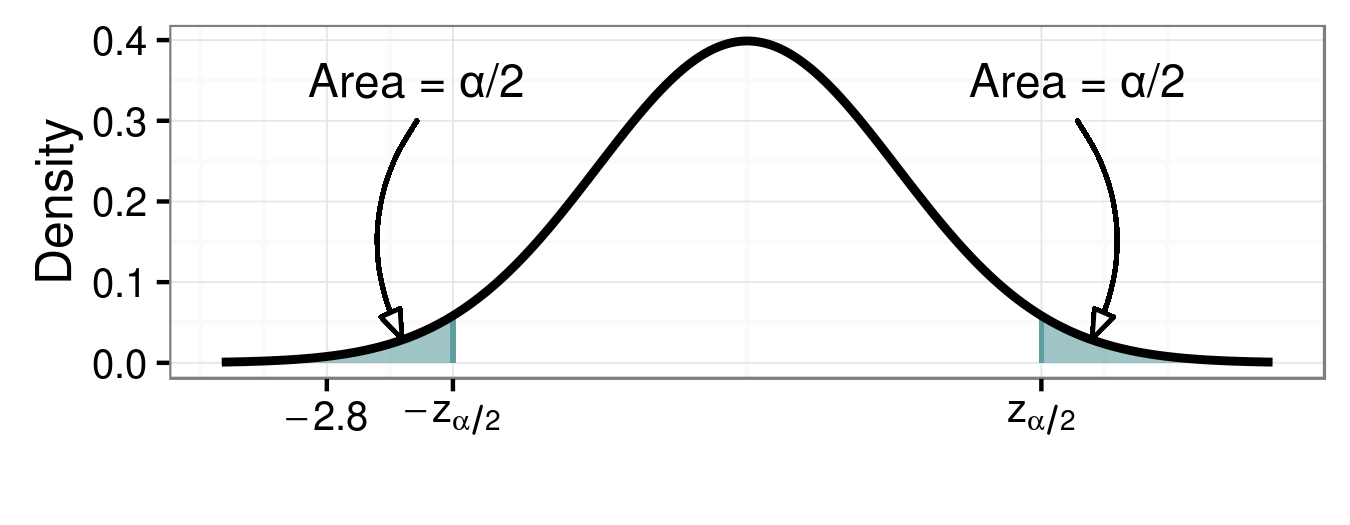
\includegraphics[width=4.5in]{../images/ch08_cv}
\par}

\end{frame}

\begin{frame}{Types of errors in hypothesis tests}
\begin{block}{}
\large
In an hypothesis test, either the null hypothesis is true or it is not, and either the null hypothesis is rejected or it is not. Thus, there are four possible outcomes.\\
\medskip
{\centering
\tabspacemed
\begin{tabular}{ r | c | c}
& Reject $H_0$ & Do not reject $H_0$\\
\hline
$H_0$ is true & Type I error ($\alpha$) & Correct decision\\
\hline
$H_0$ is not true & Correct decision & Type II error ($\beta$)
\end{tabular}
\tabspacedef
\par}
\medskip
\begin{itemize}
\pause\item A type I error occurs when the null hypothesis is rejected when it is in fact true. The probability of making a type I error in a test is designated $\alpha$.
\pause\item A type II error occurs when the null hypothesis is not rejected when it is in fact not true. The probability of making a type I error in a test is designated $\beta$.
\end{itemize}
\end{block}
\end{frame}

\begin{frame}{Types of errors in hypothesis tests, cont.}
\begin{block}{}
\large
\begin{itemize}
\item The acceptable probability of committing a type I error ($\alpha$), or level of significance,  is chosen prior to conducting a hypothesis test.
\pause\item The probability of committing a type II error ($\beta$) is determined by a number of factors, including the chosen $\alpha$ and the sample size.
\pause\item The probability of \bt{not} committing a type II error ($1-\beta$) is known as the \bt{power} of a test.
\pause\item There is a trade-off between $\alpha$ and $\beta$. Smaller $\alpha$ result in larger $\beta$ (and lower power) and vice versa.
\end{itemize}
\end{block}
\end{frame}

\begin{frame}<handout:0>{Group work}
\begin{block}{}
\large
\begin{itemize}
\item For all questions, complete part (a)
\end{itemize}
\end{block}
\end{frame}


% Section 8.2
\subsection{Testing a Claim About a Proportion}

\begin{frame}{Testing claims about population proportions}
\begin{block}{}
\large
Claims about a population proportion $p$ are tested using a sample proportion $\hat p$.\\
\medskip
Recall, sampling distributions of proportion data follow a binomial distribution which, under certain conditions, approximates a normal distribution.\\
\end{block}
\end{frame}

\begin{frame}{Test statistic for proportion tests}
\begin{block}{}
\large
Tests for population proportions use a standard normal sampling distribution. The test statistic is a $z$-score.
\[z = \frac {\hat p - p_0}{\sqrt{p_0q_0/n}}\]
where $\hat p$ is the sample proportion, $p_0$ is the population proportion under the null hypothesis, $q_0=1-p_0$ and $n$ is the sample size.
\end{block}

\end{frame}


\begin{frame}{P-values for proportion tests}
\begin{block}{}
\large
Given a $z$ test statistic, the p-value is the probability of getting $z$-scores more extreme on a standard normal distribution.
\begin{itemize}
\pause\item For two-sided test:\\ 
$H_a: p \ne p_0$, p-value = $P(Z<-z) + P(Z > z) = 2 \times P(Z > z)$
\pause\item For one-sided test:\\
$H_a: p < p_0$, p-value = $P(Z < z)$\\
$H_a: p > p_0$, p-value = $P(Z > z)$
\end{itemize}
\end{block}
\end{frame}

\begin{frame}{Requirements for a proportion test}
\begin{block}{}
\large
\begin{itemize}
\item Like all hypothesis tests, sample must be a simple random sample.\\
\item Samples of proportion data follow a binomial distribution and must satisfy the binomial requirements:
\begin{itemize}
\item Fixed number of trials
\item Trials are independent
\item Two possible outcomes (success/failure)
\item Probability of each outcome is constant
\end{itemize}
\item For the binomial to approximate a normal distribution, $np$ and $nq$ must both be at least 5.
\end{itemize}
\end{block}
\end{frame}

\begin{frame}{Steps for a proportion hypothesis test}
\begin{block}{}
\large
\begin{enumerate}
\item Identify null and alternative hypotheses from research question\\
$H_0: p = p_0$\\
$H_a: p \ne p_0, \, p < p_0, \, p> p_0$
\item Check the requirements for using normal distribution
\item Calculate $z$ test statistic
\item Calculate p-value
\item Compare p-value to significance level $\alpha$ and report decision
\item State conclusion in terms of original research question
\end{enumerate}
\end{block}
\end{frame}

\begin{frame}{Hypothesis tests for a proportion in StatCrunch}

\begin{block}{}
\large
\begin{itemize}
\item Stat $\to$ Proportion Stats $\to$ One Sample $\to$ With Summary
\item Enter ``\# of successes" and ``\# of observations"
\item Select ``Hypothesis test for p"
\item Enter the appropriate values for null and alternative hypotheses.
\item Click ``Compute!"
\item The test statistic and p-value are found in ``Z-Stat" and ``P-value"
\end{itemize}
\end{block}

\end{frame}

\begin{frame}{Hypothesis test for a proportion, example}
\begin{exampleblock}{Example}
\large
The proportion of teen drivers who text or email while driving is 40\%. A school district adds an education program for all high school students in hopes of lowering that proportion. Two months after the program, the district surveys a random sample of teen drivers. The survey finds that 62 out of 212 teens surveyed had texted or emailed while driving during the previous month. Test whether the program was successful at a 0.05 level of significance.
\begin{enumerate}
\pause\item Identify null and alternative hypotheses from research question\\
\pause$H_0: p = 0.4$\\
$H_a: p < 0.4$\\
Population: teen drivers who had attended the education program
\end{enumerate}
\end{exampleblock}
\end{frame}

\begin{frame}{Hypothesis test for a proportion, example}
\begin{exampleblock}{Example}
\large
\begin{enumerate}
\setcounter{enumi}{1}
\item Check the requirements for using normal distribution
\pause\begin{itemize}
\item Simple random sample
\item Requirements of a binomial satisfied (fixed sample size, two outcomes, independent, constant probability of success)
\item $p=0.4, \, q=0.6, \, n=212$\\
$np > 5, \, nq >5$
\end{itemize}
\pause\item Calculate $z$ test statistic\\
\pause$z = -3.1964013$
\pause\item Calculate p-value\\
\pause$p = 0.0007$
\end{enumerate}
\end{exampleblock}
\end{frame}

\begin{frame}{Hypothesis test for a proportion, example}
\begin{exampleblock}{Example}
\large
\begin{enumerate}
\setcounter{enumi}{4}
\item Compare p-value to significance level $\alpha$ and report decision\\
\pause$p = 0.0007 < \alpha =0.05$. Reject null hypothesis.

\pause\item State conclusion in terms of original research question\\
\pause There is evidence that teen drivers who attended the program text and email while driving at a lower rate than 40\%.
\end{enumerate}

\end{exampleblock}
\end{frame}

\begin{frame}<handout:0>{Group work}
\begin{block}{}
\large
\begin{itemize}
\item For questions 1 and 2, complete part (b)
\end{itemize}
\end{block}
\end{frame}

% Section 8.3
\subsection{Testing a Claim About a Mean}

\begin{frame}{Testing claims about population means}
\begin{block}{}
\large
Claims about a population mean $\mu$ are tested using a sample mean $\bar x$.\\
\medskip
Recall, if population standard deviations are unknown, sampling distributions of sample means follow a t distribution with the appropriate degrees of freedom.\\
\end{block}
\end{frame}

\begin{frame}{Test statistic for mean tests}
\begin{block}{}
\large
Tests for population means use the t sampling distribution. The test statistic is a $t$-score.
\[t = \frac {\bar x - \mu_0}{s/\sqrt{n}}\]
where $\bar x$ is the sample mean, $\mu_0$ is the population mean under the null hypothesis, $s$ is the sample standard deviation and $n$ is the sample size.
\end{block}

\end{frame}


\begin{frame}{P-values for mean tests}
\begin{block}{}
\large
Given a $t$ test statistic, the p-value is the probability of getting $t$-scores more extreme on a t distribution.
\begin{itemize}
\pause\item For two-sided test:\\ 
$H_a: \mu \ne \mu_0$, p-value = $P(T<-t) + P(T > t) = 2 \times P(T > t)$
\pause\item For one-sided test:\\
$H_a: \mu < \mu_0$, p-value = $P(T < t)$\\
$H_a: \mu > \mu_0$, p-value = $P(T > t)$
\end{itemize}
\end{block}
\end{frame}


\begin{frame}{Steps for a mean hypothesis test}
\begin{block}{}
\large
\begin{enumerate}
\item Identify null and alternative hypotheses from research question\\
$H_0: \mu = \mu_0$\\
$H_a: \mu \ne \mu_0, \, \mu < \mu_0, \, \mu> \mu_0$
\item Use a t distribution
\item Calculate $t$ test statistic
\item Calculate p-value
\item Compare p-value to significance level $\alpha$ and report decision
\item State conclusion in terms of original research question
\end{enumerate}
\end{block}
\end{frame}

\begin{frame}{Hypothesis tests for a mean in StatCrunch}

\begin{block}{}
\large
\begin{itemize}
\item Stat $\to$ T Stats $\to$ One Sample $\to$ With Summary\\ (or $\to$ With Data)
\item Enter ``Sample mean", ``Sample std. dev." and ``Sample size"\\
(or select column which contains data)
\item Select ``Hypothesis test for $\mu$"
\item Enter the appropriate values for null and alternative hypotheses.
\item Click ``Compute!"
\item The test statistic and p-value are found in ``T-Stat" and ``P-value"
\end{itemize}
\end{block}

\end{frame}

\begin{frame}{Hypothesis test for a mean, example}
\begin{exampleblock}{Example}
\large
A study is conducted of the heights of Metro State students. The heights of a sample of 35 male students are measured. The mean height from the sample is $\bar x = 68.1$ with a standard deviation of $s=3.5$. Conduct a test at $\alpha=0.05$ level of significance of the claim that male Metro State students are shorter than the general population of 69.2 inches.
\begin{enumerate}
\pause\item Identify null and alternative hypotheses from research question\\
\pause$H_0: \mu = 69.2$\\
$H_a: \mu < 69.2$\\
Population: Male Metro State students
\end{enumerate}
\end{exampleblock}
\end{frame}

\begin{frame}{Hypothesis test for a mean, example}
\begin{exampleblock}{Example}
\large
\begin{enumerate}
\setcounter{enumi}{1}

\item Use a t distribution
\pause\item Calculate $t$ test statistic\\
\pause$t=-1.8593394$
\pause\item Calculate p-value\\
\pause$p = 0.0358$
\pause\item Compare p-value to significance level $\alpha$ and report decision\\
\pause$p = 0.0358 < \alpha = 0.05$. Reject the null hypothesis.
\pause\item State conclusion in terms of original research question\\
\pause There is evidence that male Metro State students are shorter than the general population.
\end{enumerate}

\end{exampleblock}
\end{frame}

\begin{frame}{Hypothesis test for a mean, example}
\begin{exampleblock}{Example}
\large
A clinical trial of an experimental drug for a rare disease is conducted. The survival times in months of 10 patients given the new drug are below. Test the claim that the drug changes the survival time for the expected survival time of 36 months at a 0.01 level of significance.\\
\medskip
{\centering
35.5, 40.5, 44.7, 37.2, 34.7, 41.3, 37.8, 34.5, 39.8, 37.1
\par}
\begin{enumerate}
\pause\item Identify null and alternative hypotheses from research question\\
\pause$H_0: \mu = 36$\\
$H_a: \mu \ne 36$\\
Population: Patients with disease taking experiment drug
\end{enumerate}
\end{exampleblock}
\end{frame}

\begin{frame}{Hypothesis test for a mean, example}
\begin{exampleblock}{Example}
\large
\begin{enumerate}
\setcounter{enumi}{1}

\item Use a t distribution
\pause\item Calculate $t$ test statistic\\
\pause$t=2.2462$
\pause\item Calculate p-value\\
\pause$p = 0.05132$
\pause\item Compare p-value to significance level $\alpha$ and report decision\\
\pause$p = 0.05132 > \alpha = 0.01$. Do not reject the null hypothesis.
\pause\item State conclusion in terms of original research question\\
\pause There is not evidence that the experimental drug changes survival time.
\end{enumerate}

\end{exampleblock}
\end{frame}

\begin{frame}<handout:0>{Group work}
\begin{block}{}
\large
\begin{itemize}
\item For questions 3 and 4, complete part (b)
\end{itemize}
\end{block}
\end{frame}

\end{document}